\section*{\fontsize{18pt}{1}\selectfont Introduction}

\subsection*{Background}

Transmission Control Protocol (TCP) is the protocol of choice in many data centers. However, it is very sensitive to losses (by design, as a mean for congestion control), which can degrade the performance within the data centers significantly \cite{zilberman2017has}. Various congestion control and avoidance recovery mechanisms are thus of high importance in this field to minimise such loss rate. Still, not all TCP losses are born equal. For example, losses happening at the destination host's network interface card (NIC) are not an indication of congestion within the network. It is assumed that fast retransmission of such lost packets, from within the network, can increase the utilization of the network.

 In-network computing is an emerging research area in systems and networking, where applications traditionally running on the host are offloaded to the network hardware (e.g., switch, NIC). Examples of applications offloaded in the past include network functions (DNS server \cite{dns}), distributed systems functions such as consensus (P4xos \cite{p4xos}), various caching (netCache \cite{netCache}, netChain \cite{netChain}) and even a game (Tic-Tac-Toe). Key-Value Store (KVS) is also among the popular type of in-network applications. 
 
 Therefore, it is particularly interesting, and indeed challenging, to see how network-accelerated KVS concepts can be applied to TCP recovery in order to improve cross-datacentre performance.
 
 \subsection*{The Project}
 Currently, when there is packet loss, signaled by duplicate ACKs (DUP ACKs), the DUP ACKs will traverse all the way back to the host (\textbf{Figure \ref{tradition-tcp}}). The host receives the DUP ACKs, then resends the packet. The goal of my project is to implement a fast TCP recovery mechanism, which aims to reduce the response time to DUP ACKs and reduce changes to the congestion window by retransmitting packets from within the network (e.g., from the switch), instead of sending the DUP ACKs back to the host (\textbf{Figure \ref{project-tcp}}). The implementation will be based on KVS concepts, where the key is the flow Id and sequence number, and the value is the packet.
 
For this project, I will be using the P4 programming language \cite{p4.org}. It is a language designed to allow the programming of packet forwarding planes. Besides, unlike general purpose languages such as C or Python, P4 is domain-specific with a number of constructs optimized around network data forwarding, hence is well suited to such a network application. 

\vspace*{5mm}

 \begin{figure}[h]
	\centering
	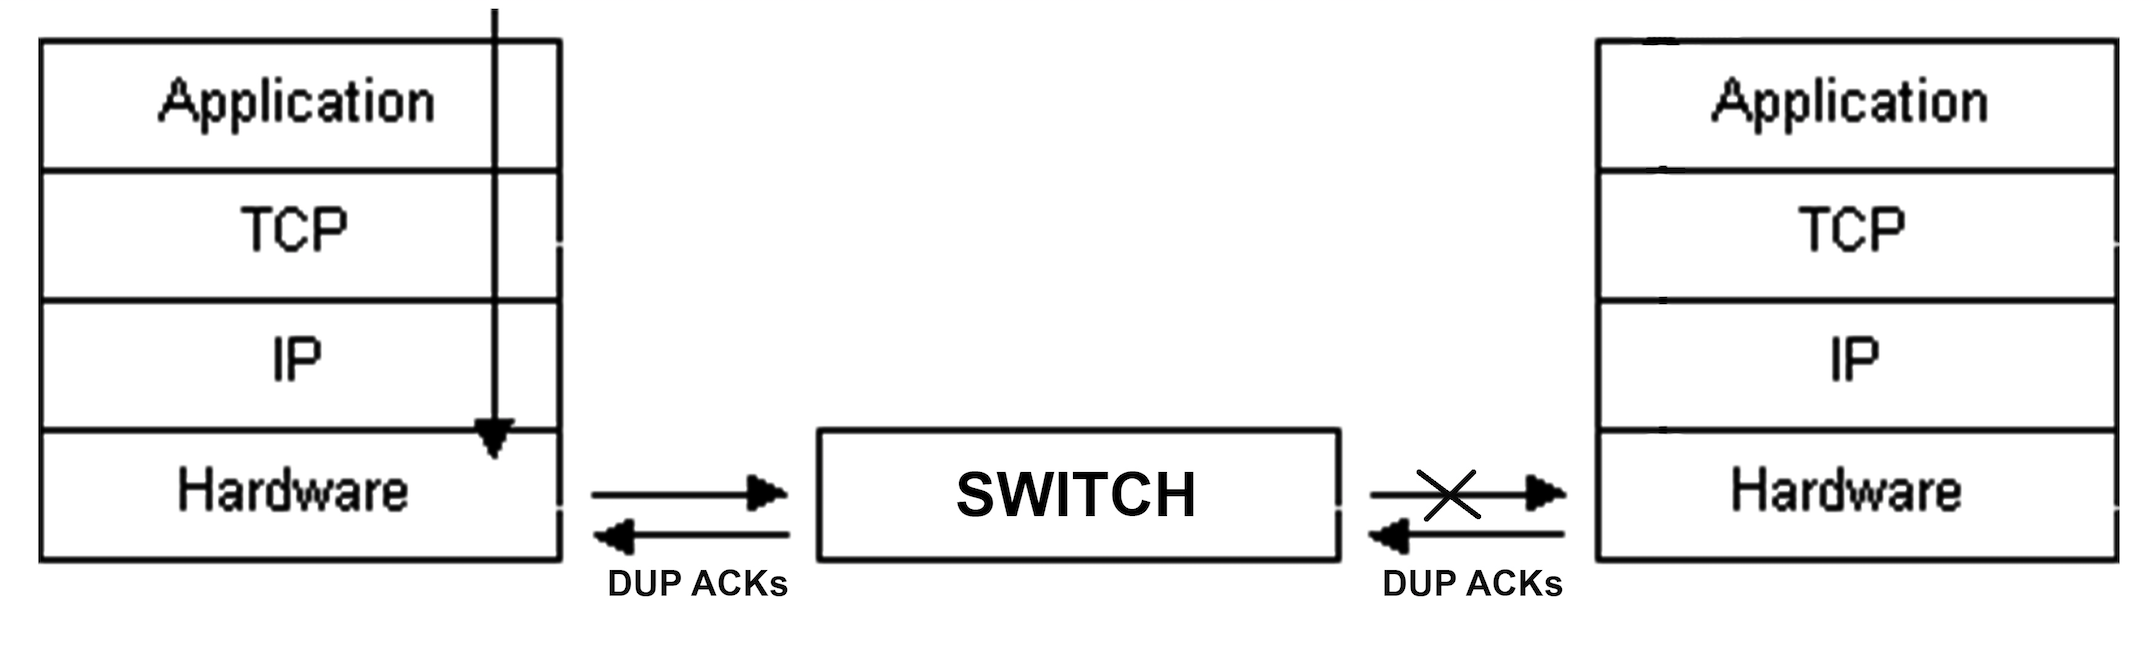
\includegraphics[width=\textwidth]{../Proposal/Figs/tradition-tcp.png}
	\caption{The standard convention of TCP handling.}
	\label{tradition-tcp}
\end{figure}

\begin{figure}[h]
	\centering
	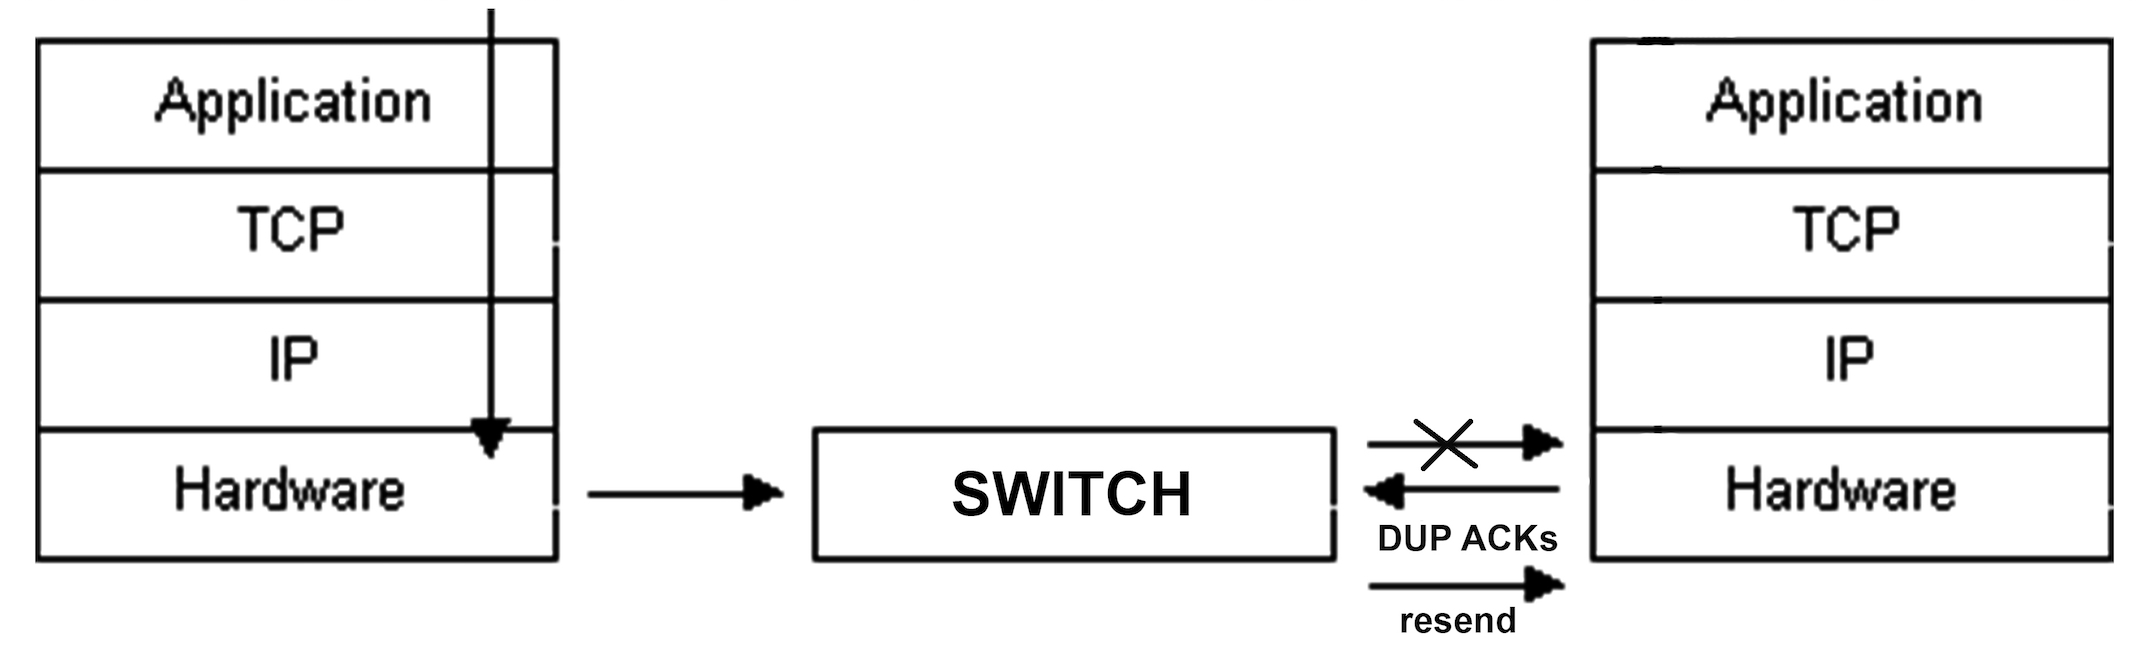
\includegraphics[width=\textwidth]{../Proposal/Figs/project-tcp.png}
	\caption{The proposed TCP handling.}
	\label{project-tcp}
\end{figure}